\documentclass[oneside]{book}
\usepackage[utf8]{inputenc}
\usepackage[T1]{fontenc}
\usepackage[icelandic]{babel}
\addto\extrasicelandic{\sisetup{locale = DE}}
\usepackage[margin=1in]{geometry}
\usepackage{lmodern}
\usepackage{amsmath}
\usepackage{amssymb}
\usepackage{amsthm}
\usepackage{tikz}
\usepackage{enumerate}
\usepackage[inline]{enumitem}
\usepackage{mathrsfs}
\usepackage{physics}
\usepackage{bm}
\usepackage{appendix}
\usepackage{lscape}
\usepackage{moreenum}
\usepackage{xcolor}
\usepackage[pdftex, hidelinks]{hyperref}
\usepackage{wrapfig}
\usepackage{graphics}
\usepackage{graphicx}
\usepackage{float}
\usepackage{tcolorbox}
\usepackage{caption}
\usepackage{subcaption}
\usepackage{dsfont}
\usepackage[separate-uncertainty=true,multi-part-units=single,output-decimal-marker={,},group-separator = {.}]{siunitx}
\usepackage{epigraph}
\usepackage{tasks}

\usepackage{import}
\usepackage{xifthen}
\usepackage{pdfpages}
\usepackage{transparent}
\usepackage{gnuplottex}

\newcommand{\incfig}[1]{%
    \def\svgwidth{\columnwidth}
    \import{./figures/}{#1.pdf_tex}
}


\theoremstyle{definition}
\newtheorem{theorem}{Lögmál}[chapter]
\newtheorem{setning}[theorem]{Regla}
\newtheorem{definition}[theorem]{Skilgreining}
\newtheorem{remark}[theorem]{Athugasemd}
\newtheorem{example}[theorem]{Dæmi}

\DeclareMathOperator\diag{diag}
\DeclareMathOperator\artanh{artanh}
\DeclareMathOperator\Det{Det}
\DeclareMathOperator\sgn{sgn}

\newcommand{\R}{\mathbb{R}}  
\newcommand{\Z}{\mathbb{Z}}
\newcommand{\N}{\mathbb{N}}
\newcommand{\Q}{\mathbb{Q}}

\newcommand{\duck}[1]{,,#1``}

\newcommand{\explain}[2]{\underbrace{#1}_\textrm{$#2$}}

\title{Eðlisfræði handa 5.~bekk eðlisfræðideildar II}
\author{Matthias Baldursson Harksen}
\date{}

\setlength\parindent{0pt}

\begin{document}

\pagestyle{empty}

\,

\vspace{5cm}

\begin{center}
    \textbf{\Huge{Eðlisfræði}}
\end{center}

\begin{center}
    \textbf{\Large{Eðlisfræðideild II}}
\end{center}


\begin{figure}[H]
    \centering
    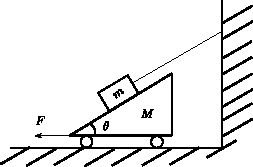
\includegraphics[scale = 2]{figures/forsidumynd.pdf}
\end{figure}

\vspace{7cm}

\begin{center}
    \textbf{\Large{Matthias Baldursson Harksen}}
\end{center}

\newpage

\tableofcontents

\chapter{Verklegar tilraunir}


Í þessum hluta munum við kynna helstu aðferðir sem við beitum í verklegri eðlisfræði. Sökum Covid-19 þurfum við að finna betri leið til þess að útfæra verklega kennslu. Ég hef því tekið saman nokkrar tilraunir fyrir ykkur til að framkvæma í heimahúsum aðeins með símana ykkar og einfaldan tækjabúnað að vopni. Til þess að framkvæma þessar tilraunir skuliði sækja forritið \verb|phyphox| sem ætti að vera aðgengilegt fyrir alla snjallsíma.

\newpage

\section{Eðlismassi pappírs}

\subsection*{Inngangur}

Í þessari tilraun ætlum við að mæla eðlismassa pappírs.

\subsection*{Tækjabúnaður}

\begin{itemize}
    \item Búnki af blöðum.
    
    \item Reglustika.
    
    \item Vog.
\end{itemize}

\subsection*{Leiðbeiningar}

Takið bunka af blöðum (það er erfitt að mæla þykktina á einu blaði). Teljið fjölda blaðsíðna, $n$, í bunkanum (einföld leið til þess er að prenta út $n$ auðar blaðsíður). Mælið rúmmál bunkans, $V = \ell b h$, með því að mæla lengdina, $\ell$, breiddina $b$ og hæðina $h$ á bunkanum. Mælið loksins massa bunkans, $m$, með voginni. Skráið allar mælingar ykkar á staðalformi ásamt óvissu.

\subsection*{Fræði}

Eðlismassi hlutar er táknaður með $\rho$. Ef eðlismassi hlutarins er einsleitur þá gildir að:
\begin{align*}
    \rho = \frac{m}{V},
\end{align*}
þar sem $m$ er massi hlutarins og $V$ er rúmmál hans. \\

Þar sem að þetta verkefni snýr aðallega að því að læra óvissureikninga þá er gott að rifja upp helstu reiknireglur varðandi óvissur. Látum $A \pm \Delta A$, $B \pm \Delta B$, $C \pm \Delta C$ og $D \pm \Delta D$ vera mælistærðir. Þá gildir að:
\begin{align*}
    \frac{A \pm \Delta A}{\left( B \pm \Delta B\right)\left( C \pm \Delta C\right)\left( D \pm \Delta D\right)} = \frac{A}{BCD} \pm \frac{A}{BCD}\left( \frac{\Delta A}{A} + \frac{\Delta B}{B} + \frac{\Delta C}{C} + \frac{\Delta D}{D} \right).
\end{align*}

\subsection*{Úrvinnsla}

\begin{enumerate}[label = (\roman*)]
    \item Hversu þykkt er eitt blað? Skilið niðurstöðunni ykkar á staðalformi ásamt óvissu.
     
    \item Hver er eðlismassi pappírs? Skilið niðurstöðunni ykkar á staðalformi ásamt óvissu.
\end{enumerate}

\newpage

\section{Skoppstuðull skopparabolta}

\subsection*{Inngangur}

Í þessari tilraun ætlum við að ákvarða skoppstuðul skopparabolta. Takið eftir að skoppstuðullinn er einnig háður fletinum sem boltinn skoppar á. Þið getið prófað að gera þessa tilraun með mismunandi gerðum af skopparaboltum til að sjá hversu ólíkir skoppstuðlar boltanna eru. Þið getið einnig prófað að sleppa sama skopparabolta á tveim mismunandi flötum, t.d. á annarsvegar parketi og hinsvegar flísum.

\subsection*{Tækjabúnaður}

\begin{itemize}
    \item Snjallsími með forritinu \verb|phyphox|
    
    \item Skopparabolti, fótbolti, handbolti, körfubolti.
\end{itemize}

\subsection*{Leiðbeiningar}

Opnið \verb|phyphox| í símanum ykkar og veljið \verb|(In)elastic collision| í valmyndinni. Leggið símann á jörðina þar sem þið ætlið að sleppa boltanum og smellið á þríhyrninginn, þ.e.~\verb|play| takkann til að hefja mælingu. Sleppið síðan boltanum úr einhverri hæð þannig að hann skoppi nálægt símanum (passið að skemma ekki símann) og þannig að fram kemur mæling á skjáinn. Niðurstöður mælingarinnar munu gefa ykkur upphafshæðina, $h_0$, sem boltanum var sleppt úr og hæðirnar $h_n$ sem boltinn náði eftir að hafa skoppað $n$ sinnum í jörðina. Þið sjáið líka tímann $t_n$ sem leið milli $(n-1)$-ta og $n$-ta skoppsins.


\subsection*{Fræði}


Skoppstuðull skopparabolta er táknaður með $\varepsilon$ og er skilgreindur þannig að
\begin{align*}
    \varepsilon := \frac{v_\text{eftir}}{v_{\text{fyrir}}},
\end{align*}
þar sem að $v_{\text{fyrir}}$ táknar hraða boltans áður en hann skoppar á jörðinni og $v_{\text{eftir}}$ táknar hraða boltans þegar hann hefur skoppað á jörðinni. Við getum umritað þessa jöfnu á eftirfarandi form
\begin{align*}
    v_\text{eftir} = \varepsilon \, v_{\text{fyrir}}.
\end{align*}
Gerum ráð fyrir því að loftmótstaðan sem verkar á skopparaboltann sé hverfandi. Með því að nota stöðujöfnurnar getum við sýnt að $v_\text{eftir} = \sqrt{2g \, h_\text{eftir}}$ og $v_\text{fyrir} = \sqrt{2g \, h_\text{fyrir}}$ en þar með höfum við að:
\begin{align*}
    \varepsilon = \frac{v_\text{eftir}}{v_{\text{fyrir}}} = \sqrt{\frac{h_\text{eftir}}{h_\text{fyrir}}}.
\end{align*}
Sem við getum umritað þannig að:
\begin{align*}
    h_\text{eftir} = \varepsilon^2 \, h_\text{fyrir}.
\end{align*}



\subsection*{Úrvinnsla}

\begin{enumerate}[label = (\roman*)]
    \item Skráið hjá ykkur hvernig skopparabolta þið eruð að vinna með.
    
    \item Gerið töflu með a.m.k.~8 ólíkum mælingum þar sem að þið skráið hæðirnar $h_\text{fyrir}$ og $h_\text{eftir}$.

\begin{table}[H]
    \centering
    \begin{tabular}{|c|c|}
    \hline
       $h_\text{fyrir} \, \, [\SI{}{cm}]$  & $h_\text{eftir} \, \, [\SI{}{cm}]$    \\ \hline
       & \\\hline
    \end{tabular}
\end{table}

\item Gerið graf af $h_\text{eftir}$ sem fall af $h_\text{fyrir}$. Er grafið línulegt?

\item Ákvarðið skoppstuðul skopparaboltans.
\end{enumerate}

\newpage

\section{Grunntónn vatnsflösku}

\begin{minipage}{\linewidth}

\begin{wrapfigure}{r}{1.5in}
\vspace{-1cm}
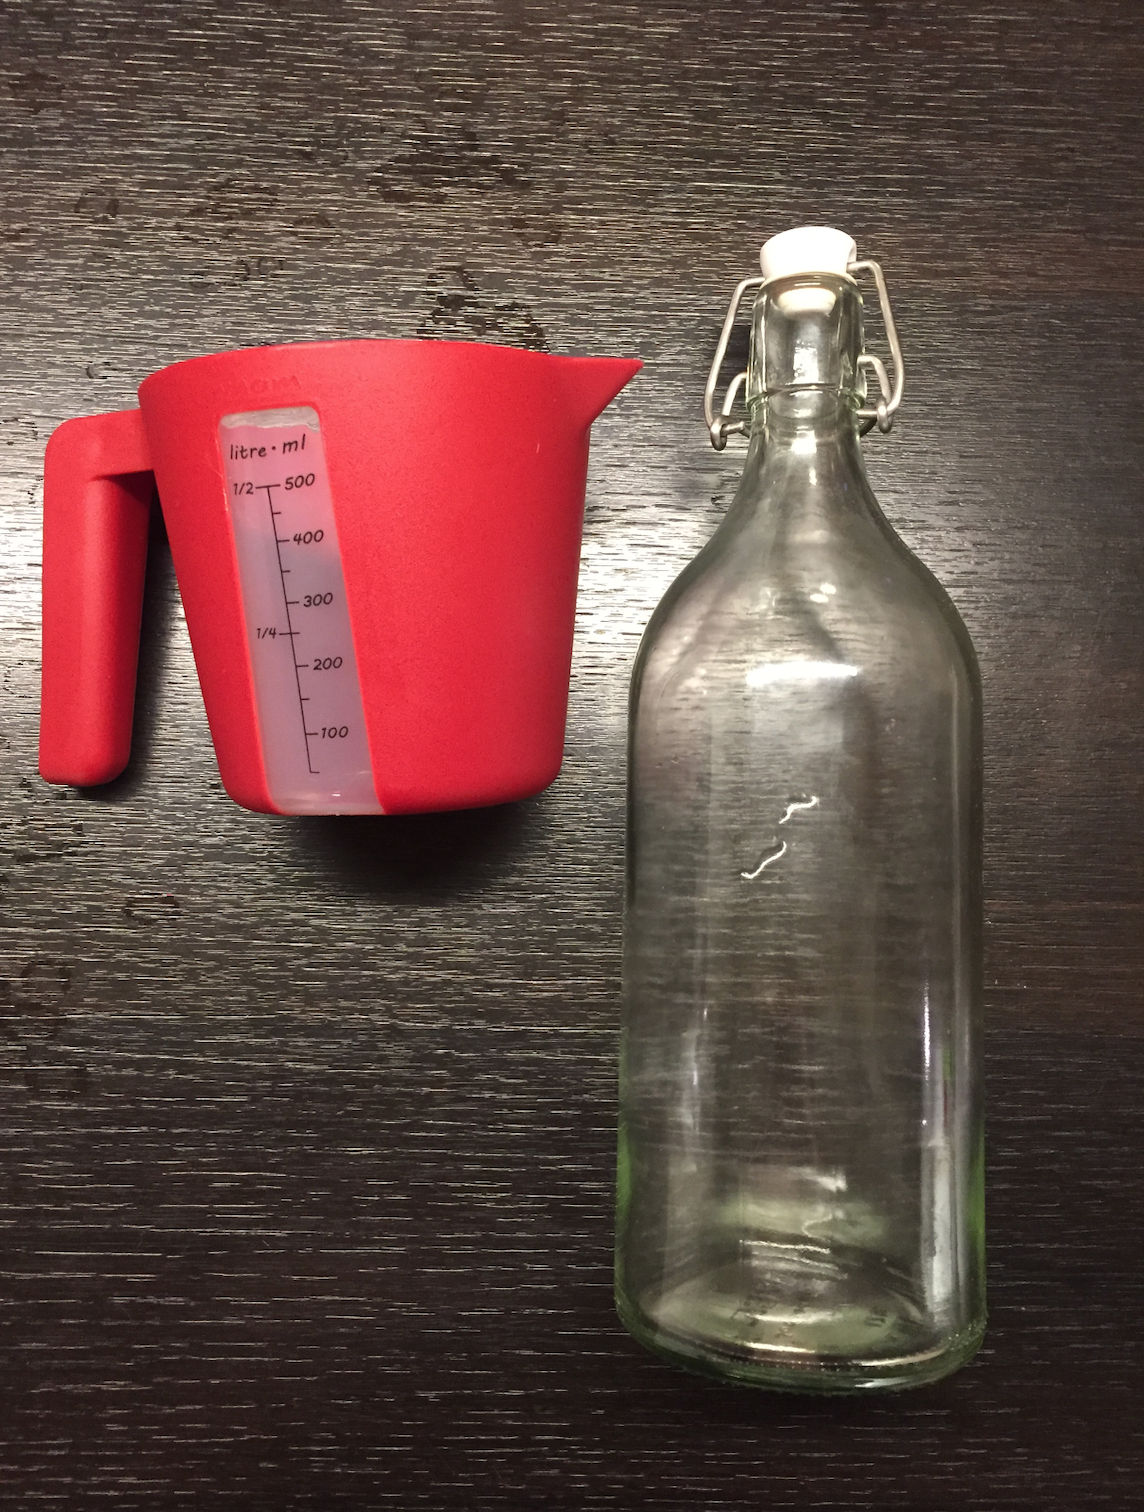
\includegraphics[width = 1.5in]{figures/hell.png}
\end{wrapfigure}

\subsection*{Inngangur}

Þegar fólk blæs á flöskustút (hornrétt á ás flöskunnar) þá heyrist blísturshljóð. Í þessari tilraun ætlum við að skoða hvernig grunntónn flösku breytist þegar við fyllum hana með vatni. Markmið okkar er að ákvarða hvernig tíðni hljóðsins sem myndast, $f$, er háð rúmmáli vatnsins, $V_{\text{vatn}}$, í flöskunni.

\subsection*{Tækjabúnaður}

\begin{itemize}
    
    \item Um það bil $\SI{1}{L}$ flaska sem hægt er að blása á stútinn á.
    
    \item Millilítramál eða vog.
    
    \item Snjallsími með forritinu \verb|phyphox|
    
    \item Reglustika, reiknivél og millimetrapappír.
\end{itemize}

\end{minipage}

\subsection*{Fræði}

Við ætlum að byrja á því að leiða út tíðni tónanna sem að myndast þegar við blásum á flöskustút. Látum þverskurðarflatarmál stútsins vera $A$ og látum hæð stútsins vera $z$. Massi loftsins í stúttnum er þá gefinn með $m = \rho_{\text{loft}} A z$ þar sem $\rho_{\text{loft}} = \SI{1.25}{kg/m^3}$ er eðlismassi loftsins. Þegar við blásum á stútinn þá fer loftið inn um vegalengd $x$ í flöskuna sjálfa og rúmmál hennar breytist þá um $Ax$. Þetta ferli er óvermið (nánar um það hvað það þýðir eftir páska) svo að við höfum eftirfarandi varðveislulögmál $PV^\gamma = \text{fasti}$ þar sem $\gamma$ er fasti sem nefnist óvermnistuðullinn. Með því að taka $\ln$ báðum meginn þá höfum við að $\ln(P) + \gamma \ln(V) = \text{fasti}$. Við athugum líka að hér er $V = V_0 - V_{\text{vatn}}$ þar sem $V$ táknar heildarrúmmálið sem er eftir í flöksunni og $V_0$ táknar upphaflega rúmmál flöskunnar áður en við byrjuðum að fylla hana með vatni. En þar með er:
\begin{align*}
    \ln(P+\Delta P) +\gamma \ln(V + \Delta V) = \ln(P) + \gamma \ln(V) \implies \ln(P) + \frac{\Delta P}{P} + \gamma \ln(V) + \gamma \frac{\Delta V}{V} = \ln(P) + \gamma \ln(V)
\end{align*}
Þar sem við höfum notað að $f(x+\Delta x) \approx f(x) + f'(x)\Delta x$. En þar með ályktum við að:
\begin{align*}
    \Delta P = - \gamma \frac{\Delta V}{V}P_0.
\end{align*}
Þar sem $P_0 = \SI{1}{atm}$. En þar með höfum við eftirfarandi kraftajöfnu:
\begin{align*}
    \rho_{\text{loft}} Az \Ddot{x} = \Delta P A = -\gamma \frac{\Delta V}{V} P_0 A = - \frac{\gamma P_0 A^2}{V_0 - V_{\text{vatn}}}x
\end{align*}
Svo við ályktum að sveiflutíðni loftsins er gefin með:
\begin{align} \label{eq:tidni}
    \omega = \sqrt{\frac{\gamma P_0 A}{\rho_{\text{loft}}z (V_0 - V_{\text{vatn}})}} \implies f = \frac{\omega }{2\pi} = \frac{1}{2\pi}\sqrt{\frac{\gamma P_0 A}{\rho_{\text{loft}}z (V_0 - V_{\text{vatn}})}}
\end{align}

\subsection*{Úrvinnsla og leiðbeiningar}

\begin{enumerate}[label = (\roman*)]
    \item Blásið á stútinn og skráið niður tíðni tónsins sem myndast með því að nota \verb|Audio Autocorrelation| í forritinu \verb|phyphox|. Hellið síðan vatni í flöskuna til að breyta tóninum og skráið hjá ykkur vatnsmagnið sem þið hafið hellt í flöskuna.
     
    \item Gerið viðeigandi graf í samræmi við jöfnu (\ref{eq:tidni}) til þess að ákvarða óvermnistuðul loftsins, $\gamma$.
\end{enumerate}

\newpage

\section{Að mæla þyngdarhröðunina}

\subsection*{Inngangur}

Í þessari tilraun ætlum við að mæla þyngdarhröðun jarðar, $g$, með aðstoð slow-motion myndavélar. \\ Við munum einnig sýna að tveir misþungir hlutir falla jafn hratt til jarðar.

\subsection*{Tækjabúnaður}

\begin{itemize}
    \item Snjallsími sem býður upp á slow motion upptökur.
    
    \item Tveir misungir hlutir til að sleppa.
    
    \item Hlutur með þekkta lengd til að hafa í bakgrunni upptökunnar, t.d.~málband eða reglustika.
    
    \item Tölva með forritinu Logger Pro.
\end{itemize}

\subsection*{Leiðbeiningar}

Takið upp slow motion myndband af tveimur hlutum sem sleppt er á sama tíma úr sömu hæð. Takið síðan upp myndband af hlut að detta með kvarða í bakgrunn (\href{https://www.dropbox.com/s/k13yf25p9ocxt9y/IMG_0976.MOV?dl=1}{sjá þetta myndband}). Setjið myndböndin inn í Logger Pro með því að velja \verb|Insert| og síðan \verb|Movie...| 
Veljið myndbandið ykkar og smellið þar næst á takka með þrem litlum rauðum punktum í neðra hægra horninu, \verb|Enable video analysis|. Veljið síðan upphafspunkt hnitakerfisins þar sem boltanum er sleppt með \verb|Set Origin| og veljið hentuga ása á hnitakerfið. Veljið síðan reglustikuna \verb|Set Scale| til að segja forritinu hvaða lengd hver díll samsvarar á myndinni. Merkið síðan inn á hvern ramma staðsetningu hlutarins með þv
í að velja \verb|Add Point|. Logger Pro ætti þá að skrá niður staðsetningu hlutarins $(x,y)$ sem fall af tíma $t$ ásamt hraða hlutarins, $(v_x, v_y)$, sem fall af tíma $t$,  miðað við hnitakerfið sem þið skilgreinduð. Myndrænar leiðbeiningar má sjá \href{https://youtu.be/rwYJV8W5_64}{í þessu myndbandi}.


\subsection*{Fræði}

Látum rammafjöldan vera táknaðan með $n$ og látum $f$ tákna fps gildi upptökunnar. Þá gildir að heildartíminn sem hefur liðið í upptökunni er gefinn með $t = n/f$. Látum $x$ tákna lárétta staðsetningu hlutarins og látum $y$ tákna lóðrétta staðsetningu hlutarins sem fall af tíma, $t$. Þá gildir samkvæmt stöðujöfnunum að:
\begin{align}
    x = x_0 + v_{x_{0}}t, \qquad \qquad y = y_0 + v_{y_{0}} t + \frac{1}{2}gt^2.
\end{align}
Þar sem $g$ táknar þyngdarhröðun jarðar, $(x_0, y_0)$ táknar upphafsstaðsetningu hlutarins og $(v_{x_{0}},v_{y_{0}} )$ táknar upphafshraða hlutarins í lárétta og lóðréttu stefnu. Þar að auki gildir samkvæmt stöðujöfnunum að lárétti hraðinn er gefinn sem fall af tíma með $v_{x} = v_{x_0}$ þar sem að engin hröðun verkar í láréttu stefnuna. Hinsvegar nýtur lóðrétti hraðinn:
\begin{align}
  v_y =   v_{y_{0}} - gt.
\end{align}

\subsection*{Úrvinnsla}

\begin{enumerate}[label = (\roman*)]
    \item Látið Logger Pro gera töflu með lóðréttri og láréttri staðsetningu hlutarins $(x,y)$, lóðréttum og láréttum hraða hlutarins, $(v_x, v_y)$, og tímanum sem hefur liðið, $t$.
    
    \item Gerið graf af lóðréttri staðsetningu hlutarins, $y$, sem fall af tíma $t$. Hver er lögun grafsins?
    
    \item Gerið graf af láréttri staðsetningu hlutarins, $x$, sem fall af tíma, $t$. Hver er lögun grafsins?
    
    \item Gerið graf af lóðréttum hraða hlutarins, $v_y$, sem fall af tíma, $t$. Hver er lögun grafsins?
    
    \item Ákvarðið þyngdarhröðun jarðar, $g$, út frá gröfunum ykkar.
\end{enumerate}

\newpage

\section{Vinnulögmálið}

\subsection*{Inngangur}

Í þessari tilraun ætlum við að sannreyna vinnulögmálið. Við ætlum að taka upp slow-motion myndband af hlut að renna meðfram láréttu yfirborði og athuga hvort að vinna núningskraftsins samræmist hreyfiorkunni sem tapaðist við færslu hlutarins.

\subsection*{Tækjabúnaður}

\begin{itemize}
    \item Snjallsími til að taka upp slow-motion myndband.
    
    \item Hlutur sem er hægt að renna meðfram láréttu yfirborði.
    
    \item Hlutur með þekkta lengd til að hafa í bakgrunni upptökunnar, t.d.~málband eða reglustika.
    
    \item Tölva með forritinu Logger Pro.
\end{itemize}

\subsection*{Leiðbeiningar}

Takið upp slow-motion myndband. Setjið myndböndin inn í Logger Pro með því að velja \verb|Insert| og síðan \verb|Movie...| 
Veljið myndbandið ykkar og smellið þar næst á takka með þrem litlum rauðum punktum í neðra hægra horninu, \verb|Enable video analysis|. Veljið síðan upphafspunkt hnitakerfisins þar sem boltanum er sleppt með \verb|Set Origin| og veljið hentuga ása á hnitakerfið. Veljið síðan reglustikuna \verb|Set Scale| til að segja forritinu hvaða lengd hver díll samsvarar á myndinni. Merkið síðan inn á hvern ramma staðsetningu hlutarins með því að velja \verb|Add Point|. Logger Pro ætti þá að skrá niður staðsetningu hlutarins $(x,y)$ sem fall af tíma $t$ ásamt hraða hlutarins, $(v_x, v_y)$, sem fall af tíma $t$,  miðað við hnitakerfið sem þið skilgreinduð.

\subsection*{Fræði}

Lítum á hlut sem hefur massa $m$ sem við ýtum af stað eftir láréttum fleti með upphafshraða $v$. Vegna núnings við yfirborðið mun hluturinn staðnæmast eftir að hann hefur runnið einhverja vegalengd $d$. Samkvæmt vinnulögmálinu höfum við þá að:
\begin{align*}
    E_{\text{fyrir}} + W_\mu = E_{\text{eftir}}
\end{align*}
Þar sem $W_\mu = -\mu mgd$ er vinna núningskraftsins þá fáum við að:
\begin{align*}
    \frac{1}{2}mv^2 - \mu mgd = 0
\end{align*}
En það þýðir einmitt að
\begin{align}
    \frac{1}{2}mv^2 = \mu mgd.
\end{align}
Við vitum einnig að hröðunin sem að massinn finnur fyrir er gefin með
\begin{align}
    a = -\mu g.
\end{align}
Við getum því fundið núningsstuðulinn milli yfirborðsins og hlutarins og þannig sannreynt vinnulögmálið.

\subsection*{Úrvinnsla}

\begin{enumerate}[label = (\roman*)]
    \item Takið upp slow motion myndband af hlut að renna meðfram yfirborði.

\item Komið myndbandinu ykkar inn í LoggerPro og greinið feril hlutarins.

\item Ákvarðið núningsstuðulinn milli hlutarins og yfirborðsins út frá lögun hraða-tíma grafsins.

\item Reiknið vinnu núningskraftsins, $W_\mu = -\mu mgd$ og berið saman við hreyfiorku hlutarins, $K = \frac{1}{2}mv^2$, rétt eftir að honum var sleppt af stað.

\end{enumerate}

\newpage

\section{Þriðja lögmál Keplers}

\subsection*{Inngangur}

Í þessari tilraun ætlum við að nota stjarnfræðiforritið Stellarium til þess að sannreyna þriðja lögmál Keplers.

\subsection*{Tækjabúnaður}

\begin{itemize}

    \item Ákjósanlegt en ekki nauðsynlegt: Forritið \href{http://stellarium.org/}{Stellarium} til að skoða sólkerfið okkar.
    
    \item Snjallsími til að horfa á myndbönd.
    
    \item Logger Pro til þess að myndgreina gögnin.
\end{itemize}

\subsection*{Leiðbeiningar}

Hlaðið niður forritinu \href{http://stellarium.org/}{Stellarium} og horfið á leiðbeiningarnar á \href{https://youtu.be/6xKXgL1irsY}{YouTube}.

\subsection*{Fræði}

Pláneturnar eru á sporbraut um sólina (eins eru tunglin á sporbraut um pláneturnar). Látum umferðartíma reikistjörnu vera táknaðann með $T$. Sporbrautir reikistjarnanna eru svo gott sem hringlaga. Látum massa plánetunnar vera gefinn með $m$ og massa sólarinnar vera $M$. Þá segir þriðja lögmál Keplers að:
\begin{align*}
    \frac{a^3}{T^2} = \frac{GM}{4\pi^2}.
\end{align*}
Þar sem að $a$ táknar langás reikistjörnunnar á sporbraut sinni um sólina, þ.e.
\begin{align*}
    a = \frac{r_{\text{min}}+r_{\text{max}}}{2}.
\end{align*}
Við getum umritað þriðja lögmálið þannig að það sé línulegt:
\begin{align} \label{eq:3Kepler}
    a^3 = \frac{GM}{4\pi^2}T^2.
\end{align}

\subsection*{Úrvinnsla}

\begin{enumerate}[label = (\roman*)]
    \item Notið Stellarium (eða myndböndin) til þess að gera töflu fyrir reikistjörnurnar:
    \begin{table}[H]
    \centering
    \begin{tabular}{|c|c|c|c|c|c|}
    \hline
       $a$ & $T$ & $a^3$ & $T^2$  \\ \hline
      & & & \\\hline
    \end{tabular}
\end{table}
    \item Gerið graf af $a^3$ sem fall af $T^2$ samkvæmt jöfnu (\ref{eq:3Kepler}) og ákvarðið massa sólarinnar með óvissu.
    \item Notið Stellarium (eða myndböndin) til þess að gera sambærilega töflu fyrir tunglin umhverfis eina af reikistjörnunum. Ákvarðið massa reikistjörnunnar með óvissu.
\end{enumerate}



\newpage




\end{document}
